\section*{Połączenie MCTS z siecią neuronową}
Algorytm Monte Carlo Tree Search w podstawowej wersji korzysta z naiwnej metody oceniającej obecny stan gry, poprzez symulację losowych ruchów aż do zakończenia gry. W grach takich jak kółko i krzyżyk, gdzie przestrzeń stanów jest bardzo ograniczona, jest to wystarczające rozwiązanie i przy odpowiedniej liczbie iteracji jest skuteczne. Natomiast w grach o dużej złożoności, jak przedstawiane szachy taki sposób oceny staje się niewystarczający. Rozwiązaniem tego problemu jest połączenie MCTS z siecią neuronową, która będzie w stanie ocenić obecny stan gry oraz przedstawić rozkład prawdopodobieństwa wszystkich następnych ruchów. Takie podejście wymaga stworzenia dwóch oddzielnych sieci, lub jednej z dwoma rozgałęzieniami. Jak było wspomniane wczęsniej, jedna z nich będzie odpowiedzialna za ocenę obecnego stanu gry (value network), a druga za wybór najlepszego ruchu (policy network).

\section*{Architektura sieci neuronowej}

\section*{Implementacja MCTS oraz integracja z siecią neuronową}
W celu integracji MCTS z siecią neuronową, funkcja UCT została zastąpioną PUCT (Predictor + UCT). Takie samo podejście zostało zastosowane w AlphaZero. Różnica między UCT a PUCT występuje w obliczaniu eksploracji, gdzie między innymi jest uwzględniana wartość prawdopodobieństwa ruchu $P(s,a)$ oraz prawdopodobieństwa wygranej (wartość stanu) $W(s,a)$ zwracane przez sieć neuronową.

\hspace{2cm}

\begin{equation}
\operatorname{PUCT}(s,a) \,=\, \widehat{Q}(s,a) \, + \, c_{\mathrm{puct}}\, P(s,a)\, \frac{\sqrt{\sum_{b} N(s,b)}}{1 + N(s,a)}\, ,
\quad
\widehat{Q}(s,a) \,=\, \dfrac{W(s,a)}{N(s,a)}\,
\end{equation}

\noindent gdzie:
\begin{description}
  \item[$\widehat{Q}$] - średnia wartość akcji $a$ w stanie $s$
  \item[$N(s)$] - liczba odwiedzin stanu $s$
  \item[$N(s,a)$] - liczba odwiedzeń akcji $a$ w stanie $s$
  \item[$\sum_{b} N(s,b)$] - suma odwiedzin wszystkich akcji w stanie $s$
  \item[$P(s,a)$] - prawdopodobieństwo wyboru akcji $a$ w stanie $s$ zwracane przez sieć neuronową
  \item[$c_{puct}$] - współczynnik eksploracji
  \item[$W(s,a)$] - wartość sumy nagród akcji $a$ w stanie $s$
\end{description}

\hspace{2cm}

Dodatkowo składnik eksploatacji jest dodatkowo normalizowany i odwracany. Odwrócenie jest konieczne ze względu na fakt, że wartość jest zawsze liczona dla przeciwnika niezależnie od tego czy obecenie jest tura białych czy czarnych. Z tego powodu zależy nam na minimalizacji tej wartości, tak aby osłabiać przeciwnika. Normalizacja do przedziału [0,1] jest konieczna ze względu na fakt, że wartość $Q$ w przypadku przeważającej liczby przegranych partii może przyjmować wartości ujemne. Dodatkowo przedział [0,1] jest bardziej intuicyjny i łatwiejszy do połączenia z wartością eksploracji.

\begin{equation}
\widehat{Q}(s,a) \,=\,
\begin{cases}
0, & N(s,a) = 0 \\
1 - \dfrac{Q(s,a) + 1}{2}, & N(s,a) > 0
\end{cases}
\end{equation}

% W ATCH THE U NOBSERVED : A S IMPLE A PPROACH TO PARALLELIZING MONTE CARLO TREE SEARCH
\section*{Zrównoleglenie MCTS}
Frameworki do tworzenia sieci neuronowych takie jak wykorzystywany PyTorch, preferują operacje na dużych partiach danych. Do teraz opisywane drzewo ruchów działało w sposób sekwencyjny. Skutkiem tego jest przetwarzanie tylko jednej próbki na raz. Karty graficzne są zoptymalizowane do wykonywania operacji na dużych macierzach, a nie na pojedynczych wektorach.

\section*{Opis działania}
W celu zrównoleglenia MCTS została wykorzystana metoda batchowania danych. Polega ona na sekwencyjnym zapisywaniu najbardziej obiecujących liści do bufora w danym stanie drzewa. Gdy taki liść zostanie dodany, zostaje wywołana na nim blokada, tak aby wymusić wybór innego liścia. Gdy bufor osiągnie określony rozmiar, lub algorytm osiągnie zakładaną ilość iteracji, są one przekazywane do sieci neuronowej w jednej partii w celu uzyskania prawdopodobieństwa wygranej oraz rozkładu prawdopodobieństwa ruchów. Po uzyskaniu wyników, drzewo jest aktualizowane poprzez wsteczną popagację oraz zostają usunięte wszystkie blokady z obliczanych liści. W ostatnim kroku, drzewo jest rozbudowywane o nowe węzły, które zostały zwrócone przez sieć neuronową.

\section*{WU-UCT - Watch the Unobserved}
Powyższy proces wybierania liści, nie jest w pełni optymalny, gdyż blokowane są tylko ostatnie węzły. Oznacza to, że zbiór potencjalnych liści ogranicza się tylko do węzłów jednego, najlepszego rodzica, gdyż algorytm cały czas schodzi w dół drzewa tylko jedną ścieżką. Rozwiązaniem tego roblemu jest wykorzystanie metody "Watch the Unobserved". Wprowadza ona zmodyfikowaną funkcję PUCT, która modyfikuje wartość eksploracji o zmienną $O_s$, przechowującą liczbę trwających obliczeń w danej gałęzi, czyli liczbę liści które są w buforze. Dzięki tak zmodyfikowanej funkcji, algorytm podczas zapełniania bufara, nabiera charakteru bardziej eksploracyjnego i wybiera liście z różnych gałęzi drzewa, a nie tylko z jednej.

Mechanizm blokowania przedstawiony w poprzednim podrozdziale, w WU-UCT pełni rolę tylko zabezpieczenia. Zapewnia on, że do bufora nie zostanie dodany ten sam liść. Z takim mechanizmem, w najgorszym przypadku dodamy najlepszy liść tego samego rodzica, który nie znajduje się w buforze.

\begin{equation}
\operatorname{WU-UCT}(s,a) \,=\, \widehat{Q}(s,a) \, + \, c_{\mathrm{puct}}\, P(s,a)\, \frac{\sqrt{(\sum_{b} N(s,b)) + O_s}}{(1 + N(s,a)) + O_s}\, ,
\end{equation}
\noindent gdzie:
\begin{description}
  \item[$\widehat{Q}$] - średnia wartość akcji $a$ w stanie $s$
  \item[$N(s)$] - liczba odwiedzin stanu $s$
  \item[$N(s,a)$] - liczba odwiedzeń akcji $a$ w stanie $s$
  \item[$\sum_{b} N(s,b)$] - suma odwiedzin wszystkich akcji w stanie $s$
  \item[$P(s,a)$] - prawdopodobieństwo wyboru akcji $a$ w stanie $s$ zwracane przez sieć neuronową
  \item[$c_{puct}$] - współczynnik eksploracji
  \item[$O_s$] - liczba trwających obliczeń węzłów potomnych stanu $s$
\end{description}

Na poniższym listingu można zauważyć bardzo dużą różnicę między samym blokowaniem wybranych liści, a blokowaniem wraz z wzorem WU-UCT. Druga metoda zapewnia dużą różnorodność wybranych ścieżek w drzewie co jest korzystne dla eksploracji.

\begin{lstlisting}[
    language=Python,
    caption=Adresy rodziców liści znajdujących się w buforze,
    inputencoding=utf8,
    basicstyle=\ttfamily\footnotesize,
    backgroundcolor=\color{gray!10},
    frame=single,
    showspaces=false,
    showstringspaces=false,
    numbers=none
]
0x705d41c78440
0x705d41c78440
0x705d41c78440
0x705d41c78440
0x705d41c78440
0x705d41c78440
0x705d41c78440
0x705d41c78440

0x7a5e5d1e1be0
0x7a5e5d1e38f0
0x7a5e5d1f1640
0x7a5e5d1f3350
0x7a5e5d0010a0
0x7a5e5d002db0
0x7a5e5d00cb00
0x7a5e5d00e810
\end{lstlisting}

\section*{Wada i zaleta WU-UCT}
Podobnie jak w biznesie, w algorytmie MCTS kluczowe jest znalezienie balansu między eksploracją, a eksploatacją. WU-UCT skupia się bardziej na eksploracji, co pozwala niekiedy wyjść z lokalnego optimum. Jednakże w przypadku zbyt dużej eksploracji, algorytm może być mniej skuteczny, gdyż skupia się na potencjalnie dobrych ruchach, a nie na najlepszych. 

Python jest językiem interpretowanym, przez co niespodziewanym wąskim gardłem są najprostrze operacje na drzewie, przez co zyskany czas na zrównolegleniu nie jest tak ogromny. Czasami występują przypadki, gdzie bardziej opłaca się czasowo iteracyjnie podążać za najlepszym liściem, niż równolegle rozwijać drzewo w szerz.

\begin{figure}[!h]
\centering
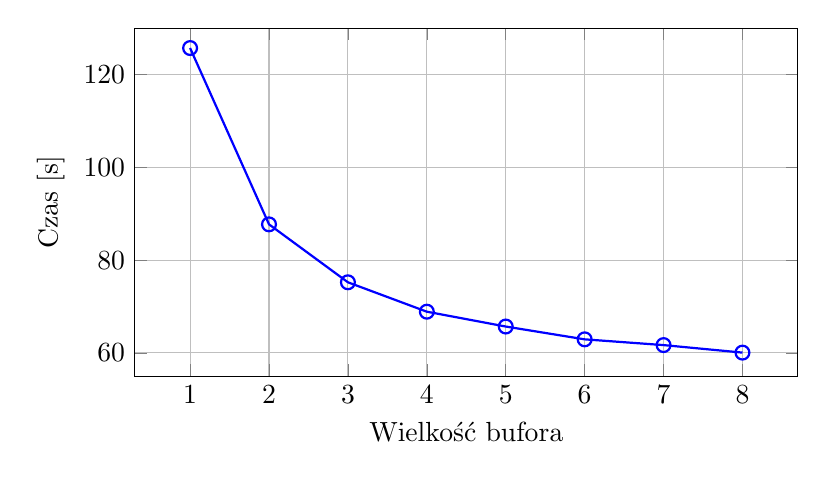
\begin{tikzpicture}
  \begin{axis}[
      width=10cm,
      height=6cm,
      grid=both,
      xlabel={Wielkość bufora},
      ylabel={Czas [s]},
      xtick={1,2,3,4,5,6,7,8},
      ymin=55,
      ymax=130,
      ymajorgrids=true,
      xmajorgrids=true,
      legend style={at={(0.02,0.98)},anchor=north west,font=\small},
      mark size=2.5pt
  ]
    \addplot+[blue, thick, mark=o] coordinates {
      (1,125.73)
      (2,87.72)
      (3,75.23)
      (4,68.89)
      (5,65.69)
      (6,62.93)
      (7,61.69)
      (8,60.07)
    };
  \end{axis}
\end{tikzpicture}
\caption{Wpływ wielkości bufora na czas wykonania 6000 iteracji}
\label{fig:metric-iteracje}
\end{figure}

Testy wydajnościowe przedstawione na wykresie zostały przeprowadzone na procesorze i7-11800H oraz GPU RTX 3060. Można łatwo zauważyć, że wraz ze wzrostem wielkości bufora, zysk czasowy jest coraz mniejszy i najoptymalniejszym rozmiarem jest 2. Taki stan rzeczy jest głównie spowodowany wymienionym wyżej Pythonem, gdzie operacje utrzymujące drzewo są kosztowne. Szczególnie jest to widoczne przy etapie ekspansji, gdzie czas wykonania wynosi $O(n * m)$, gdzie $n$ to wielkość bufora, a $m$ to liczba możliwych ruchów z danego stanu. Rozwiązaniem jest zrównoleglenie również i tego procesu, aczkolwiek jest to niemożliwe, gdyż drzewo jest zapisywane w sposób obiektowy. Podczas przekazywania danych do procesów, są one najpierw serializowane co powoduje problem z referencjami.